\documentclass[a4paper,11pt]{memoir}

\ifpdf
\usepackage[utf8]{inputenc}
\usepackage[T1]{fontenc}
\fi

%\usepackage{german}
%\usepackage[english]{babel}
%\usepackage[german]{translator}
%\usepackage{hyperref}

% This is the only file needed for actually using the smart-thesis style.
%
% Smart Thesis LaTeX template
%
% [To underline the amateurish flavour of this template, let's start with some
% nifty ASCII-Art (http://www.network-science.de/ascii/)...]
%
%      #######
%    /       ###
%   /         ##                                          #
%   ##        #                                          ##
%    ###                                                 ##
%   ## ###      ### /### /###     /###   ###  /###     ########
%    ### ###     ##/ ###/ /##  / / ###  / ###/ #### / ########
%      ### ###    ##  ###/ ###/ /   ###/   ##   ###/     ##
%        ### /##  ##   ##   ## ##    ##    ##            ##
%          #/ /## ##   ##   ## ##    ##    ##            ##
%           #/ ## ##   ##   ## ##    ##    ##            ##
%            # /  ##   ##   ## ##    ##    ##            ##
%  /##        /   ##   ##   ## ##    /#    ##            ##
% /  ########/    ###  ###  ### ####/ ##   ###           ##
%/     #####       ###  ###  ### ###   ##   ###           ##
%|
% \)
%
%
%  /###           /  /
% /  ############/ #/                              #
%/     #########   ##                             ###
%#     /  #        ##                              #
% ##  /  ##        ##
%    /  ###        ##  /##      /##       /###   ###        /###
%   ##   ##        ## / ###    / ###     / #### / ###      / #### /
%   ##   ##        ##/   ###  /   ###   ##  ###/   ##     ##  ###/
%   ##   ##        ##     ## ##    ### ####        ##    ####
%   ##   ##        ##     ## ########    ###       ##      ###
%    ##  ##        ##     ## #######       ###     ##        ###
%     ## #      /  ##     ## ##              ###   ##          ###
%      ###     /   ##     ## ####    /  /###  ##   ##     /###  ##
%       ######/    ##     ##  ######/  / #### /    ### / / #### /
%         ###       ##    ##   #####      ###/      ##/     ###/
%                         /
%                        /
%                       /
%                      /
%
% About:
% ======
%
% This template is a re-implementation of the "classicthesis" template by André
% Miede. However, it uses the "memoir" class as a basis, eliminating most
% of the external packages required by "classicthesis" and thus (hopefully)
% achieving a higher compatibility with other LaTeX packages. Large parts of
% the code have been adapted (ransacked) from André Miedes code.
%
% You can find more information about "classicthesis" at CTAN:
%
% https://www.ctan.org/pkg/classicthesis
%
% More information about the "memoir" package can be found here:
%
% https://www.ctan.org/pkg/memoir
%
%
% Authors:
% ========
%
% Jan Philip Göpfert, Andreas Stöckel
%
%
% License:
% ========
%
% This LaTeX template is published under the Creative Commons Zero license. To
% the extent possible under law, the authors have waived all copyright and
% related neighboring rights to Smart Thesis. This work is published from:
% Germany.
%


%
% EXTERNAL PACKAGES
%
\usepackage[usenames,dvipsnames,svgnames]{xcolor}
\usepackage{ragged2e} % for marginnote

%\usepackage{listings}

%
% FONT DEFINITIONS
%

% Use the following code for XeLaTeX
\ifxetex

% Setup microtype for XeLaTeX
\usepackage[expansion=false,final]{microtype}

% Load the texgyrepagella font as main font and set the ``mathpazo'' font as
% math font
\usepackage{fontspec}
\usepackage{mathpazo}
\setmainfont%
	[%
		BoldFont       = texgyrepagella-bold.otf,
		ItalicFont     = texgyrepagella-italic.otf,
		BoldItalicFont = texgyrepagella-bolditalic.otf,
		Ligatures      = TeX
	]%
	{texgyrepagella-regular.otf}

% Define a new 'widespaced' font that is used in section headings
% or chapter titles. For backwards compatibility reasons this uses
% the old calling convention \newfontfamily\fontname[<options>{font}
% instead of the newer \newfontfamily\fontname{font}[<options>]
\newfontfamily\widespaced[%
	LetterSpace=15,%
	WordSpace={1.25, 1.25, 1.25}%
]{texgyrepagella-regular.otf}%

\DeclareRobustCommand{\spacedallcaps}[1]{%
	{\widespaced\oldstylenums{\MakeTextUppercase{#1}}}%
}%
\DeclareRobustCommand{\spacedlowsmallcaps}[1]{%
	{\widespaced\oldstylenums{\textsc{\MakeTextLowercase{#1}}}}%
}%
\fi

% Use the following code for pdfLaTex
\ifpdf

% Setup microtype for pdfLaTex
\usepackage[final,tracking=true,kerning=true,spacing=nonfrench]{microtype}


\usepackage[sc]{mathpazo}

\DeclareRobustCommand{\spacedallcaps}[1]{\textls[160]{\oldstylenums{\textsc{\MakeTextUppercase{#1}}}}}%
\DeclareRobustCommand{\spacedlowsmallcaps}[1]{\textls[80]{\oldstylenums{\textsc{\MakeTextLowercase{#1}}}}}%
\fi

% Increase linespread for Palatino
\renewcommand{\linespread}{1.05}

%
% COLOR DEFINITIONS
%

\definecolor{smartgray}{gray}{0.55}
\definecolor{smartred}{HTML}{800000}
\definecolor{smartplum}{HTML}{47294F}
\definecolor{smartblue}{HTML}{193A6B}
\definecolor{smartorange}{HTML}{AA4C00}
\definecolor{smartgreen}{HTML}{3C7705}
\definecolor{smartbutter}{HTML}{A08300}

\definecolor{tangored}{HTML}{CC0000}
\definecolor{tangoplum}{HTML}{75507B}
\definecolor{tangoblue}{HTML}{3465A4}
\definecolor{tangoorange}{HTML}{F57900}
\definecolor{tangogreen}{HTML}{73D216}
\definecolor{tangobutter}{HTML}{EDD400}

\definecolor{shadecolor}{gray}{0.95}

\colorlet{heading}{smartgray}
\colorlet{ref}{smartblue}
\colorlet{cite}{smartgreen}
\colorlet{url}{smartred}
\colorlet{caption}{black}
\colorlet{margincaption}{caption}

%
% SECTIONING STYLES (toledo)
%

% See http://tex.stackexchange.com/questions/161577/memoir-hangnum-chapter-number-in-right-margin-switch for the inspiration

\setsecnumdepth{subsection}

\makeatletter
\makechapterstyle{toledo}{%
	\chapterstyle{default}

	\renewcommand*{\chapterheadstart}{\vspace*{0.0cm}}

	\renewcommand*{\chapnumfont}{\normalfont\color{heading}\addfontfeature{SizeFeatures={Size=110}}}
	\newfont{\chapterNumber}{eurb10 scaled 7000}
	\renewcommand*{\chapnumfont}{\chapterNumber\color{heading}}
	\renewcommand*{\printchaptername}{}
	\renewcommand*{\chapternamenum}{}
	\renewcommand*{\printchapternum}{%
		\raisebox{0pt}[0pt][0pt]{%
		\makebox[0pt][l]{%
		\makebox[\dimexpr\textwidth+5.45em\relax][l]{%
			\parbox[t]{\textwidth}{\mbox{}}%
			\parbox[t]{5.45em}{\hfill\chapnumfont \thechapter}}}}}%
	\renewcommand*{\chapternamenum}{}
	\renewcommand*{\afterchapternum}{}

	\renewcommand*{\afterchaptertitle}{%
	\par\parbox{\textwidth}{\hrulefill}\par%
	\vspace*{4ex}}
	\renewcommand*{\chaptitlefont}{\normalfont\large}
	\renewcommand*{\printchaptertitle}[1]{%
		\parbox[b]{\textwidth}{%
			\raggedright\chaptitlefont\spacedallcaps{##1}%
		}%
	}

	\setsecheadstyle{\spacedlowsmallcaps}
	\setsecindent{-3.5ex}
	\setbeforesecskip{-4ex plus -1ex minus -.2ex}
	\setaftersecskip{4ex plus 1ex minus .2ex}

	\setsubsecheadstyle{\itshape}
	\setbeforesubsecskip{-4ex plus -1ex minus -.2ex}
	\setaftersubsecskip{4ex plus 1ex minus .2ex}
	\setsecnumformat{\spacedlowsmallcaps{\csname the##1\endcsname\quad}}

%	\setparaheadstyle{\normalsize\itshape}

	\renewcommand*{\abstractnamefont}{\spacedlowsmallcaps}
}
\makeatother

\chapterstyle{toledo}

%
% FIGURES
%

\captionstyle{\small}
\captionnamefont{\slshape\color{caption}}

\newsubfloat{figure}% Create subfloat in figure environment
\newsubfloat{table}% Create subfloat in table environment

%
% ACKNOWLEDGEMENT
%

\makeatletter
\newcommand{\acknowledgementname}{Acknowledgements}
\newenvironment{acknowledgement}{%
  \setup@bstract
  \if@bsrunin\else
    \ifnumber@bs \num@bs \else
      \begin{\absnamepos}\abstractnamefont\acknowledgementname\end\absnamepos%
      \vspace{\abstitleskip}%
    \fi
  \fi
  \put@bsintoc%
  \begin{@bstr@ctlist}\if@bsrunin\@bsrunintitle\fi\abstracttextfont}%
  {\par\end{@bstr@ctlist}}

\newcommand{\smartcopyright}[1]{\begingroup%
	\pagebreak%
	\thispagestyle{empty}%
	\footnotesize%
	\par\vspace*{\fill}%
	\hspace{-1.1cm}%
	\parbox{10cm}{%
		\noindent%
		Copyright \textcopyright\ \the\year\ \applytolist[, ]{}{\@author}\\[0.5cm]%
		{#1}%
	}%
\endgroup}

\newcommand{\smartinitialepigraph}[2]{\begingroup
	\cleardoublepage
	\thispagestyle{empty}
	\vspace*{2cm}
	\epigraph{#1}{#2}
	\cleardoublepage
\endgroup}

\let\oldepigraph\epigraph
\renewcommand{\epigraph}[2]{\oldepigraph{#1}{\spacedlowsmallcaps{#2}}}

\makeatother

%
% MARGINNOTE
%

%
% There are three commands for placing elements in the margin:
%
% \marginnote{<TEXT>}
% Just like \marginpar but with correct formating
%
% \marginfig{<SHORT CAPTION>}{<FIGURE CONTENT>}{<LONG CAPTION>}{\label{<LABEL>}}
% \margintbl{<SHORT CAPTION>}{<TABLE CONTENT>}{<LONG CAPTION>}{\label{<LABEL>}}
% Places a figure/table in the margin
% - <SHORT CAPTION> is the caption as it occurs in the list of figures/tables
% - <FIGURE CONTENT>/<TABLE CONTENT> is the actual figure/table content
% - <LONG CAPTION> is the caption below the figure
% - <LABEL> is the label -- we decided to let you explicitly type "\label" here
% as this allows LaTeX editors to index the label and provide auto completion.
%

% Define the "marginnote" command. For compatibility reasons
% we do not override marginpar.
\strictpagecheck
\newcommand{\marginnote}[1]{\hspace*{0pt}\marginpar{
	\microtypesetup{disable}%
	\slshape\footnotesize%
	\vspace*{-0.725em}%
	\checkoddpage%
	\ifoddpage%
		\RaggedRight%
	\else%
		\RaggedLeft%
	\fi%
	{#1}%
	\microtypesetup{enable}%
}\ignorespaces}

\newcommand{\marginfloat}[8]{\marginnote{{#1}%
\par\refstepcounter{#4}\textcolor{margincaption}{#5 #6}: {#2}#3}%
\addcontentsline{#7}{#4}{\protect\numberline {#6}{\ignorespaces #8}}\ignorespaces}

\newcommand{\marginfig}[4]{\marginfloat{#2}{#3}{#4}{figure}{Figure}{\thefigure}{lof}{#1}}
\newcommand{\margintbl}[4]{\marginfloat{#2}{#3}{#4}{table}{Table}{\thetable}{lot}{#1}}

%
% PAGE STYLE (headers, footers)
%

\makeatletter

% Deactivate capitalization of headers.
\nouppercaseheads

% Define the new "berlin" style.
\makepagestyle{berlin}

% Display the page number in the footer.
\makeevenfoot{berlin}{\thepage}{}{}
\makeoddfoot{berlin}{}{}{\thepage}

% Override the chapter style with the unfinished "berlin" style
% to eliminate the header and to make sure a consistent footer
% style is used.
\copypagestyle{chapter}{berlin}

% Define the "berlin" style
\makepsmarks{berlin}{%
	\def\chaptermark##1{%
	\markboth{\memUChead{%
		\ifnum \c@secnumdepth >\m@ne
		\if@mainmatter
			\@chapapp\ \thechapter. \ %
		\fi
		\fi
		##1}}{}}%
	\def\tocmark{\markboth{\memUChead{\contentsname}}{\memUChead{\contentsname}}}%
	\def\lofmark{\markboth{\memUChead{\listfigurename}}{\memUChead{\listfigurename}}}%
	\def\lotmark{\markboth{\memUChead{\listtablename}}{\memUChead{\listtablename}}}%
	\def\bibmark{\markboth{\memUChead{\bibname}}{\memUChead{\bibname}}}%
	\def\indexmark{\markboth{\memUChead{\indexname}}{\memUChead{\indexname}}}%
	\def\sectionmark##1{%
	\markright{\memUChead{%
		\ifnum \c@secnumdepth > \z@
		\thesection. \ %
		\fi %
		##1}}}}
\makepsmarks{berlin}{%
	\createmark{chapter}{left}{nonumber}{}{}
	\createmark{section}{right}{shownumber}{}{\ }
	\createplainmark{toc}{both}{\contentsname}
	\createplainmark{lof}{both}{\listfigurename}
	\createplainmark{lot}{both}{\listtablename}
	\createplainmark{bib}{both}{\bibname}
	\createplainmark{index}{both}{\indexname}
	\createplainmark{glossary}{both}{\glossaryname}
}

% Discriminate between "oneside" and "twoside" documents.
\if@twoside
	\makeevenhead{berlin}{\spacedlowsmallcaps{\leftmark}}{}{}
	\makeoddhead{berlin}{}{}{\spacedlowsmallcaps{\rightmark}}
\else
	\makeoddhead{berlin}{\spacedlowsmallcaps{\rightmark}}{}{}
\fi

% Use the berlin style.
\pagestyle{berlin}

\makeatother

%
% FOOTNOTES
%

\footmarkstyle{\textsc{#1}}
\setlength{\footmarkwidth}{-0.5em}
\setlength{\footmarksep}{0.5em}
\setlength{\footparindent}{0em}

%
% EPIGRAPHS
%
\makeatletter

% Make the epigraph span two third of the text width
\setlength{\epigraphwidth}{0.66\textwidth}

% Disable the rule below the epigraph
\setlength{\epigraphrule}{0pt}

% Use the normal font size
\epigraphfontsize{\normalsize}

% Style the epigraph itself -- use italic text and
% flush it to the right
\newenvironment{epigraphstyle}{
%	\microtypesetup{disable}%
	\small\slshape%
%	\RaggedLeft%
}{%
%	\microtypesetup{enable}%
}
\epigraphtextposition{epigraphstyle}

% Style the epigraph source -- prepend it with a em-dash
% and make sure no indentation is added after the epigraph
\newenvironment{epigraphsourcestyle}%
{%#
	--- \small\raggedleft\color{smartred}%
}{%
	\@afterindentfalse\@afterheading%
}
\epigraphsourceposition{epigraphsourcestyle}

\makeatother

%
% TITLEPAGE
%

\makeatletter
\newcommand\thesistype[1]{\renewcommand\@thesistype{#1}}
\newcommand\@thesistype{}

\newcommand\discipline[1]{\renewcommand\@discipline{#1}}
\newcommand\@discipline{}

\newcommand\institution[1]{\renewcommand\@institution{#1}}
\newcommand\@institution{}

\newcommand\supervisors[1]{\renewcommand\@supervisors{#1}}
\newcommand\@supervisors{}

\newcommand\reviewers[1]{\renewcommand\@reviewers{#1}}
\newcommand\@reviewers{}

\newcommand\internalid[1]{\renewcommand\@internalid{#1}}
\newcommand\@internalid{}

\newcommand\subtitle[1]{\renewcommand\@subtitle{#1}}
\newcommand\@subtitle{}

\newcommand{\applytolist}[3][{,\\\vspace{0.1cm}}]{%
	\def\nextitem{\def\nextitem{#1}}%
	\@for \el:=#3\do{\nextitem{#2{\el}}}%
}

\newcommand{\smarttitle}{
{\begingroup
\thispagestyle{empty}
\makeatletter
\raggedright
\vfill
{\LARGE \spacedallcaps{\@thesistype} \\}
{\Large \spacedlowsmallcaps{\@discipline}\\}
\vfill
{\huge \textcolor{smartred}{\spacedallcaps{\@title}}\\}
\vspace{3mm}
{\LARGE \textcolor{smartred}{\spacedallcaps{\@subtitle}}\\}
\vfill
{\LARGE \applytolist{\spacedallcaps}{\@author}\\}
\vfill
{\Large \applytolist{\itshape}{\@institution}}
\vfill
{\Large \spacedlowsmallcaps{Reviewed by}\\}
\vspace{0.1cm}
{\large \applytolist{\spacedallcaps}{\@reviewers}}
\vfill
{\Large \spacedlowsmallcaps{Supervised by}\\}
\vspace{0.1cm}
{\large \applytolist{\spacedallcaps}{\@supervisors}}
\vfill
\vfill
{\Large \spacedlowsmallcaps{\today} \hfill \spacedlowsmallcaps{\@internalid}}
\vfill
\makeatother
\endgroup}}

\makeatletter
%
% PAGE LAYOUT
%
\settypeblocksize{23.45cm}{11.85cm}{*}
%\setlength{\textheight}{23.45cm}
%\setlength{\textwidth}{11.85cm}
\setlrmargins{3.141592653589793cm}{*}{*}
\setulmargins{*}{*}{*}
\setmarginnotes{0.8cm}{3.5cm}{1cm}
\checkandfixthelayout


% Contains some packages which are commonly used in a thesis.
% Note that these are optional.
\usepackage{csquotes} % Context sensitive quotation facilities. Recommended by babel and should be loaded before babel.

\usepackage[english]{babel} % Sets the language used. Essential for proper hyphenation. Translates key words like 'figure' or 'table'. Note that 'english' is American English.

\usepackage{latexsym,amsmath,amssymb,amsthm,amscd} % Provides math enviroments, math symbols and more things useful for math.

\usepackage{mathtools} % Enhances amsmath and provides further mathematical tools.

\usepackage{graphicx} % Provides inclusion of graphics and a proper interface for '\in­clude­graph­ics'.
% Su­per­sedes 'epsfig' and 'graphics'.

\usepackage{enumitem} % Provides control over list environments. Supersedes 'enumerate', which gives enumerate environment an optional argument which determines the style in which the counter is printed.

%\let\newfloat\undefined % Hack to make floatrow work with memoir.
%\usepackage{floatrow} % Handles alignment of floats (figures), with centering as default.

\usepackage{xspace} % Ugly hack that sometimes helps with otherwise missing spaces.

\usepackage[backgroundcolor=white,linecolor=smartblue,bordercolor=smartblue,textsize=footnotesize]{todonotes} % Todo notes.

% Use sans-serif font in todos to clearly distinguish it from other text
\makeatletter
\renewcommand{\todo}[2][]{\@bsphack\@todo[#1]{\sffamily{#2}}\@esphack\ignorespaces}
\makeatother

\usepackage[style=alphabetic,backend=biber]{biblatex} % Bibliography.

%\usepackage{algorithm} % Algorithms.
% Use default Memoir floats for algorithms
\newcommand{\algorithmname}{Algorithm}
\newcommand{\listalgorithmname}{List of Algorithms}
\newlistof{listofalgorithms}{loa}{\listalgorithmname}
\newfloat[chapter]{algorithm}{loa}{\algorithmname}
\newfixedcaption{\falgcaption}{algorithm}
\newlistentry[chapter]{algorithm}{loa}{0}
\cftsetindents{algorithm}{0em}{2.3em}
\makeatletter
\g@addto@macro\insertchapterspace{\addtocontents{loa}{\protect\addvspace{10pt}}}
\makeatother

%\usepackage{algpseudocode} % Algorithms.

\usepackage{varioref} % Automatically locates references on other pages. Load before hyperref.

%\usepackage[hidelinks]{hyperref} % Clickable references.
\usepackage[pdfencoding=auto,pdfborderstyle={/S/U/W 1},linkbordercolor=ref,colorlinks,linkcolor=ref,citecolor=cite,urlcolor=url]{hyperref} % Clickable references.

\usepackage[all]{hypcap} % Anchors links to the beginning of their respective floats. Load after hyperref.

\usepackage[noabbrev,capitalize,nameinlink]{cleveref} % Names references automatically. Load after hyperref.

\usepackage[toc,acronym]{glossaries} % Glossary.

\usepackage{booktabs}
\usepackage{multirow}

\usepackage{pgfplots}
\pgfplotsset{compat=1.8}
\pgfplotscreateplotcyclelist{smart}{%
  tangoplum,semithick,every mark/.append style={fill=tangoplum!80!black},mark=*\\%
  tangogreen,semithick,every mark/.append style={fill=tangogreen!80!black},mark=square*\\%
  tangoorange,semithick,every mark/.append style={fill=tangoorange!80!black},mark=otimes*\\%
  tangoblue,semithick,mark=star\\%
  tangobutter,semithick,every mark/.append style={fill=tangobutter!80!black},mark=diamond*\\%
  tangored,semithick,every mark/.append style={solid,fill=tangored!80!black},mark=*\\%
}
\pgfplotsset{cycle list name=smart}

\usepackage{listings}

\definecolor{mygreen}{rgb}{0,0.6,0}
\definecolor{mygray}{rgb}{0.5,0.5,0.5}
\definecolor{mymauve}{rgb}{0.58,0,0.82}

\lstset{ %
  backgroundcolor=\color{white},   % choose the background color; you must add \usepackage{color} or \usepackage{xcolor}
  basicstyle=\footnotesize,        % the size of the fonts that are used for the code
  breakatwhitespace=false,         % sets if automatic breaks should only happen at whitespace
  breaklines=true,                 % sets automatic line breaking
  captionpos=b,                    % sets the caption-position to bottom
  commentstyle=\color{mygreen},    % comment style
  deletekeywords={...},            % if you want to delete keywords from the given language
  escapeinside={\%*}{*)},          % if you want to add LaTeX within your code
  extendedchars=true,              % lets you use non-ASCII characters; for 8-bits encodings only, does not work with UTF-8
  frame=single,	                   % adds a frame around the code
  keepspaces=true,                 % keeps spaces in text, useful for keeping indentation of code (possibly needs columns=flexible)
  keywordstyle=\color{blue},       % keyword style
  language=C++,                	% the language of the code
  otherkeywords={*,...},           % if you want to add more keywords to the set
  numbers=left,                    % where to put the line-numbers; possible values are (none, left, right)
  numbersep=5pt,                   % how far the line-numbers are from the code
  numberstyle=\tiny\color{mygray}, % the style that is used for the line-numbers
  rulecolor=\color{black},         % if not set, the frame-color may be changed on line-breaks within not-black text (e.g. comments (green here))
  showspaces=false,                % show spaces everywhere adding particular underscores; it overrides 'showstringspaces'
  showstringspaces=false,          % underline spaces within strings only
  showtabs=false,                  % show tabs within strings adding particular underscores
  stepnumber=1,                    % the step between two line-numbers. If it's 1, each line will be numbered
  stringstyle=\color{mymauve},     % string literal style
  tabsize=2,	                   % sets default tabsize to 2 spaces
  title=\lstname,                   % show the filename of files included with \lstinputlisting; also try caption instead of title
  literate=%
    {Ö}{{\"O}}1
    {Ä}{{\"A}}1
    {Ü}{{\"U}}1
    {ß}{{\ss}}1
    {ü}{{\"u}}1
    {ä}{{\"a}}1
    {ö}{{\"o}}1
    {~}{{\textasciitilde}}1
}

\renewcommand{\lstlistingname}{Quellcode}


% Contains some macros which are commonly used in a thesis.
% Note that these are optional.
% Abbreviations
\newcommand*{\eg}{e.\,g.\@\xspace}
\newcommand*{\ie}{i.\,e.\@\xspace}
\newcommand*{\cf}{cf.\@\xspace}
\newcommand*{\etal}{et.\@ al.\@\xspace}
%\newcommand*{\etc}{etc.\@\xspace}
\makeatletter
\newcommand*{\etc}{%
  \@ifnextchar{.}%
    {etc}%
      {etc.\@\xspace}%
}
\makeatother

% Sets
\newcommand*{\R}{\mathbb{R}}
\newcommand*{\Q}{\mathbb{Q}}
\newcommand*{\Z}{\mathbb{Z}}
\newcommand*{\N}{\mathbb{N}}

% Matrix/vector operations
\newcommand*{\transpose}[1]{{#1^{\top}}}
\newcommand*{\inverse}[1]{{#1^{-1}}}
\newcommand*{\conjugate}[1]{{#1^{\ast}}}
\newcommand*{\pseudoinverse}[1]{{#1^{+}}}

% Stochastics
\newcommand*{\probability}[1]{{\mathrm{Pr}{#1}}}
\newcommand*{\expectation}[1]{{#1}}

% Optimization
\DeclareMathOperator*{\argmax}{arg\,max}
\DeclareMathOperator*{\argmin}{arg\,min}
\DeclareMathOperator{\lb}{lb}
\DeclareMathOperator{\sign}{sgn}

% These packages are only used in the demo and not necessarily
% required for smart-thesis.
\usepackage{todonotes}

% Loads bibliography for citations.
\addbibresource{thesis-bibliography.bib}

% Starts creation of a glossary.
\makeglossaries
\newglossaryentry{handle}{
	name=Handle,
	plural=Handles,
	description={Eine GPU-Hardwareadresse. In mancher Literatur wird der Begriff Handle auch für die \gls{glid} benutzt, in dieser Arbeit werden jedoch die Begrifflichkeiten der offiziellen Spezifikationen genutzt}
}
\newglossaryentry{glid}{
	name=Object Name,
	plural=Object Names,
	description={Der eindeutige Name, mit dem OpenGL einen Buffer o.Ä. identifiziert. Für gewöhnlich ein unsigned integer}
}
\newglossaryentry{ubum}{
	name=UBUM,
	plural=UBUMs,
	description={Uniform Buffer Unified Memory. Eine OpenGL-Erweiterung von Nvidia, die es ermöglicht, \glspl{ubo} bindless zu benutzen}
}
\newglossaryentry{ubo}{
	name=UBO,
	plural=UBOs,
	description={Uniform Buffer Object. Eine in OpenGL 3.1 eingeführte Technik, die die Verwendung von persistenten Uniforms mit Hilfe von Buffern ermöglicht}
}
\newglossaryentry{vbum}{
	name=VBUM,
	plural=VBUMs,
	description={Vertex Buffer Unified Memory. Eine OpenGL-Erweiterung von Nvidia, die es ermöglicht, Vertexattribute bindless zu benutzen}
}
\newglossaryentry{vbo}{
	name=VBO,
	plural=VBOs,
	description={Vertex Buffer Object. Eine in OpenGL x.x eingeführte Technik. Muss seit OpenGL y.y zwangsweise mit \glspl{vao} verwendet werden}
}
\newglossaryentry{vao}{
	name=VAO,
	plural=VAOs,
	description={Vertex Array Object. Eine Datenstruktur, welche Metainformationen zur Verwendung von \glspl{vbo} enthält}
}
\newglossaryentry{bind}{
	name=bind,
	plural=binden,
	description={Ein essentieller Vorgang in OpenGL. Durch das Binden einer Datenstruktur wird OpenGL angewiesen, diese für \glspl{dc} zu nutzen}
}
\newglossaryentry{dc}{
	name=Drawcall,
	plural=Drawcalls,
	description={Ein essentieller Vorgang in OpenGL. Ein Drawcall weisst OpenGL an, ein Objekt mit Hilfe eines Shaders unter Berücksichtigung von Uniforms, Vertexattributen und Texturen zu zeichnen}
}
\newglossaryentry{culling}{
	name=Culling,
	description={Eine Technik, bei der Objekte, die sich nicht im Frustum befinden und damit nicht im Bild auftauchen werden, OpenGL nicht zum Zeichnen übergeben werden, um eine höhere Performance zu erreichen}
}
\newglossaryentry{ft}{
	name=Frametime,
	description={Die Zeit, die ein Renderer benötigt, um ein einzelnes Bild zu zeichnen, das Inverse von \gls{fps}}
}
\newglossaryentry{lft}{
	name=LFT,
	description={Longest Frame Time. Die maximale Zeit, die ein Renderer benötigt, um ein einzelnes Bild zu zeichnen}
}
\newglossaryentry{target}{
	name=Target,
	description={Ein Target ist ein besonderer Binding Point für Buffer, da er nur \todo{stuff}}
}
\newglossaryentry{vertexattrib}{
	name=Vertexattribut,
	plural=Vertexattribute,
	description={Ein Vertexattribut kann alles sein, was einen Vertex definiert, etwa seine Position, Normalenvektor oder Farbe}
}
\newglossaryentry{cl}{
	name=Clientstate,
	description={Ein Clientstate ist ein bestimmter Zustand, den \todo{stuff}}
}
\newglossaryentry{bindless}{
	name=Bindless,
	description={Bindless ist ein {azdo}-Ansatz, bei dem Objekte (\glspl{ubo}, \glspl{vbo}, \etc) nicht mehr gebunden, sondern nurnoch den Shadern ,,verfügbar gemacht`` werden}
}
\newglossaryentry{azdo}{
	name=AZDO,
	description={,,Approaching Zero Driver Overhead`` hat zum Ziel, besonders CPU-lastige Szenen zu beschleunigen, indem Abstraktion von der Hardware verringert oder sogar aufgehoben wird}
}
\newglossaryentry{resident}{
	name=resident,
	description={Eine \gls{handle} oder ein Objekt resident zu machen bedeutet, OpenGL mitzuteilen, dass dieses Objekt in naher Zukunft gebraucht wird und deshalb in den Speicher geladen und dort vorgehalten werden sollte. Eine \gls{handle} oder ein Objekt nonresident zu machen bedeutet hingegen, dass OpenGL freigestellt wird, dieses Objekt aus dem Speicher zu entfernen, etwa um Platz für andere, gerade benötigte Objekte zu machen}
}
\newglossaryentry{fps}{
	name=FPS,
	description={Frames per Second - die Anzahl an Bildern die ein Programm innerhalb einer Sekunde zeichnet}
}
\newglossaryentry{texunit}{
	name=Texture Unit,
	plural=Texture Units,
	description={Eine Texture Unit ist ein Platz, an dem eine Textur auf der GPU gespeichert werden kann. Die Anzahl der Texture Units ist stark begrenzt}
}



% Define all the metadata to be listed in \smarttitle and \smartcopyright
\thesistype{Master Thesis}
\discipline{Intelligent Systems}
\title{TBD Master Thesis Title}
\author{Robert Feldhans}
\institution{University of Bielefeld,Technical Faculty,AG TBD}
\supervisors{Prof.\@~Dr.\@~TDB,M.Sc.\@~Birte Carlmeyer,M.Sc.\@~Florian Flier}
%\internalid{M13}

\begin{document}

\frontmatter

\smarttitle

%%!TEX root = thesis.tex

%=============================================================================


\chapter{Abstract}
- First introduction to speech recognition and related stuff

- then presentation of our pipeline, which is based on two pillars.

- Then evaluation based on two experiments to show the validity of this approach and performance of the proposed pipeline.

- Lastly we will discuss further work, improvements to the proposed pipeline, additional things to evaluate

\newpage

\tableofcontents

\mainmatter
%!TEX root = thesis.tex

\chapter{Introduction \& Motivation}
\label{motiv:start}
In order to be accepted by humans, social robots in general depend on \gls{hri} \cite{6926324}, which in turn is influenced and shaped by human-human interaction \cite{mediaequation}.
Since speech is one of the most important modalities of communication between humans, it is no surprise that it is also one of the most important parts of \gls{hri}.
In \gls{hri}, verbal dialogue can be divided into speech generation and the main interest of this thesis: speech understanding.

Being able to perfectly recognize the words a person spoke does not completely cover speech understanding, e.g. the perception and engagement of the speaker \cite{Ivaldi2017}.
An exemplary dialogue between a robot and two humans is depicted in a provided video\footnote{\url{https://www.youtube.com/watch?v=iEMKZdwJPE8}} and in stills in figure \ref{pic:moti:imustgonow}.
The video depicts parts of a RoboCup@home Task at the RoboCup World Championship 2018 in Montreal.
In three different instances two referees are giving a robot commands, but they take turns in speaking to the robot.
The robot does not recognize two different speakers, and thus, cannot react appropriately.
More so:
when asking for the confirmation of a specific command, it does not even seem to recognize that a different person gives this confirmation, or that the original referee walked away and no longer partakes in the conversation.

\begin{figure}[]
	\centering
	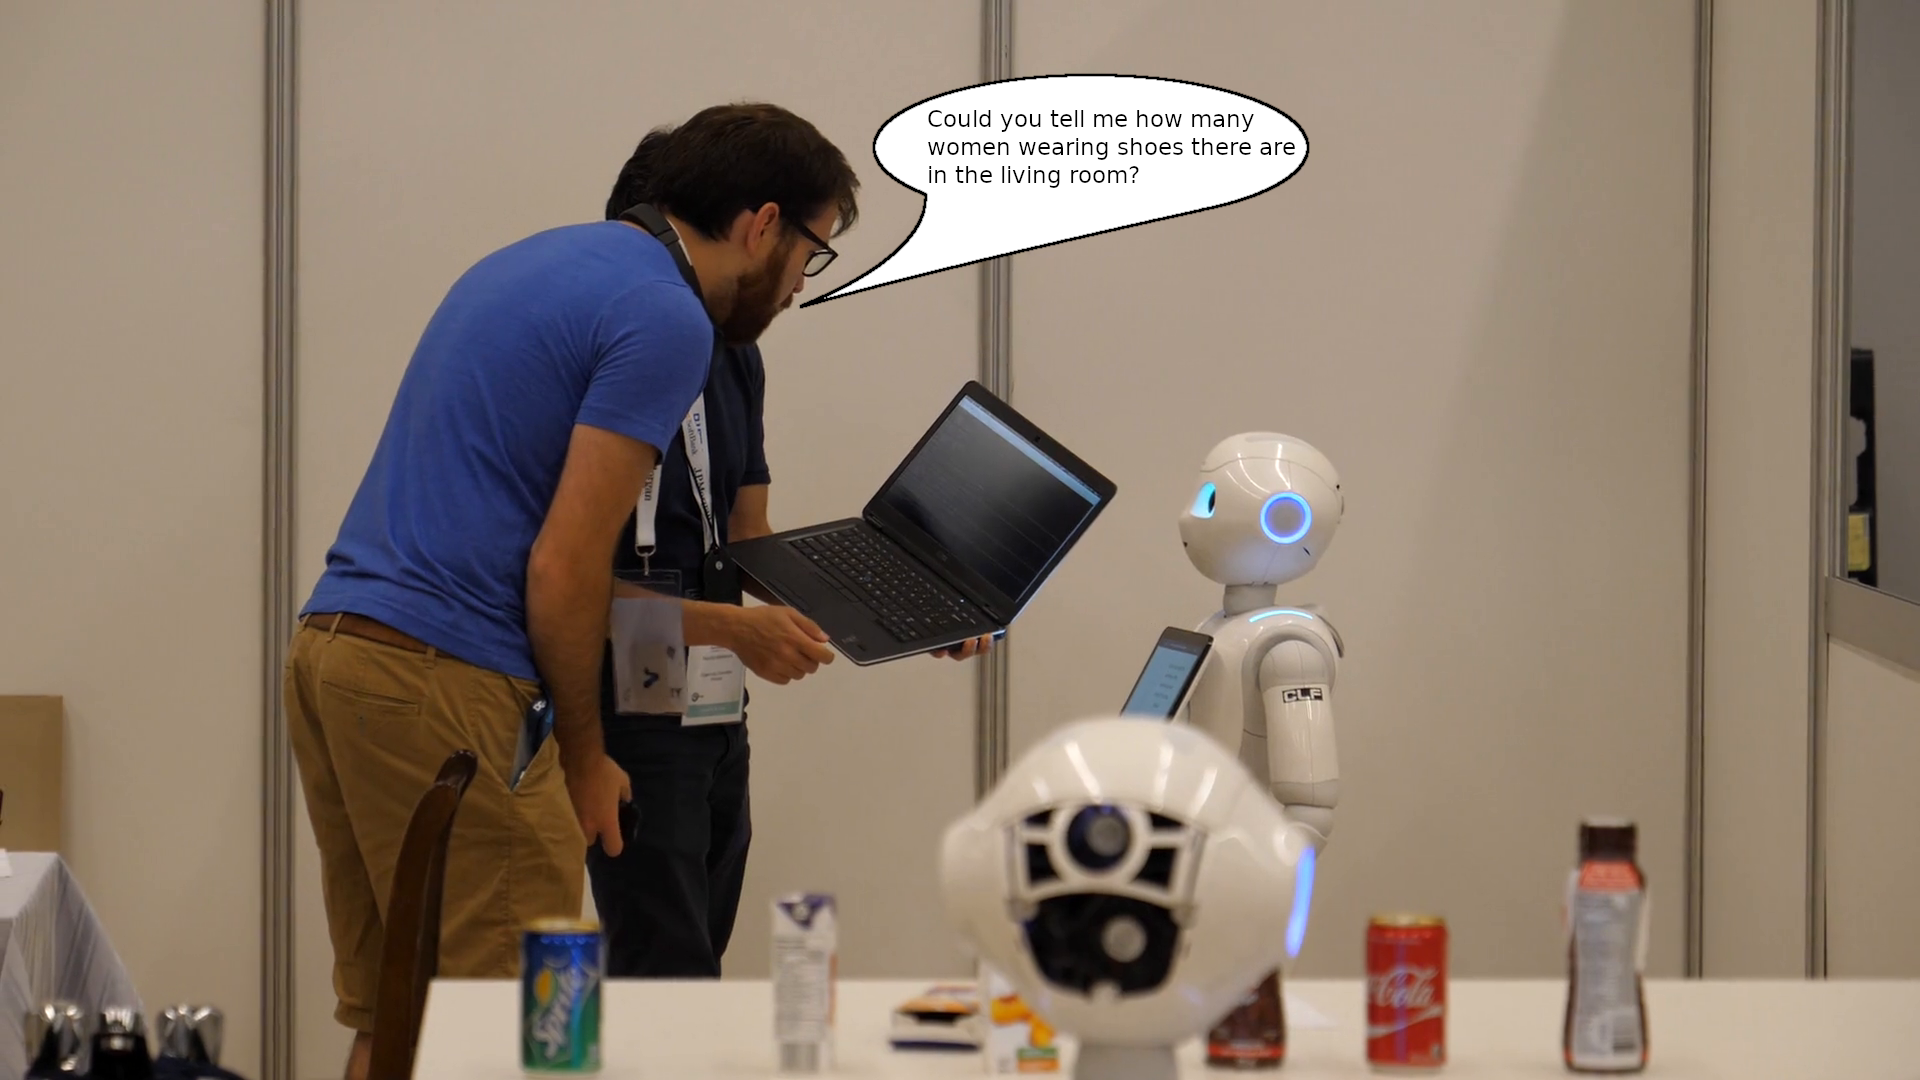
\includegraphics[width=.8\textwidth]{bilder/motivation/intro_1_edit.png}\\\vspace{3pt}
	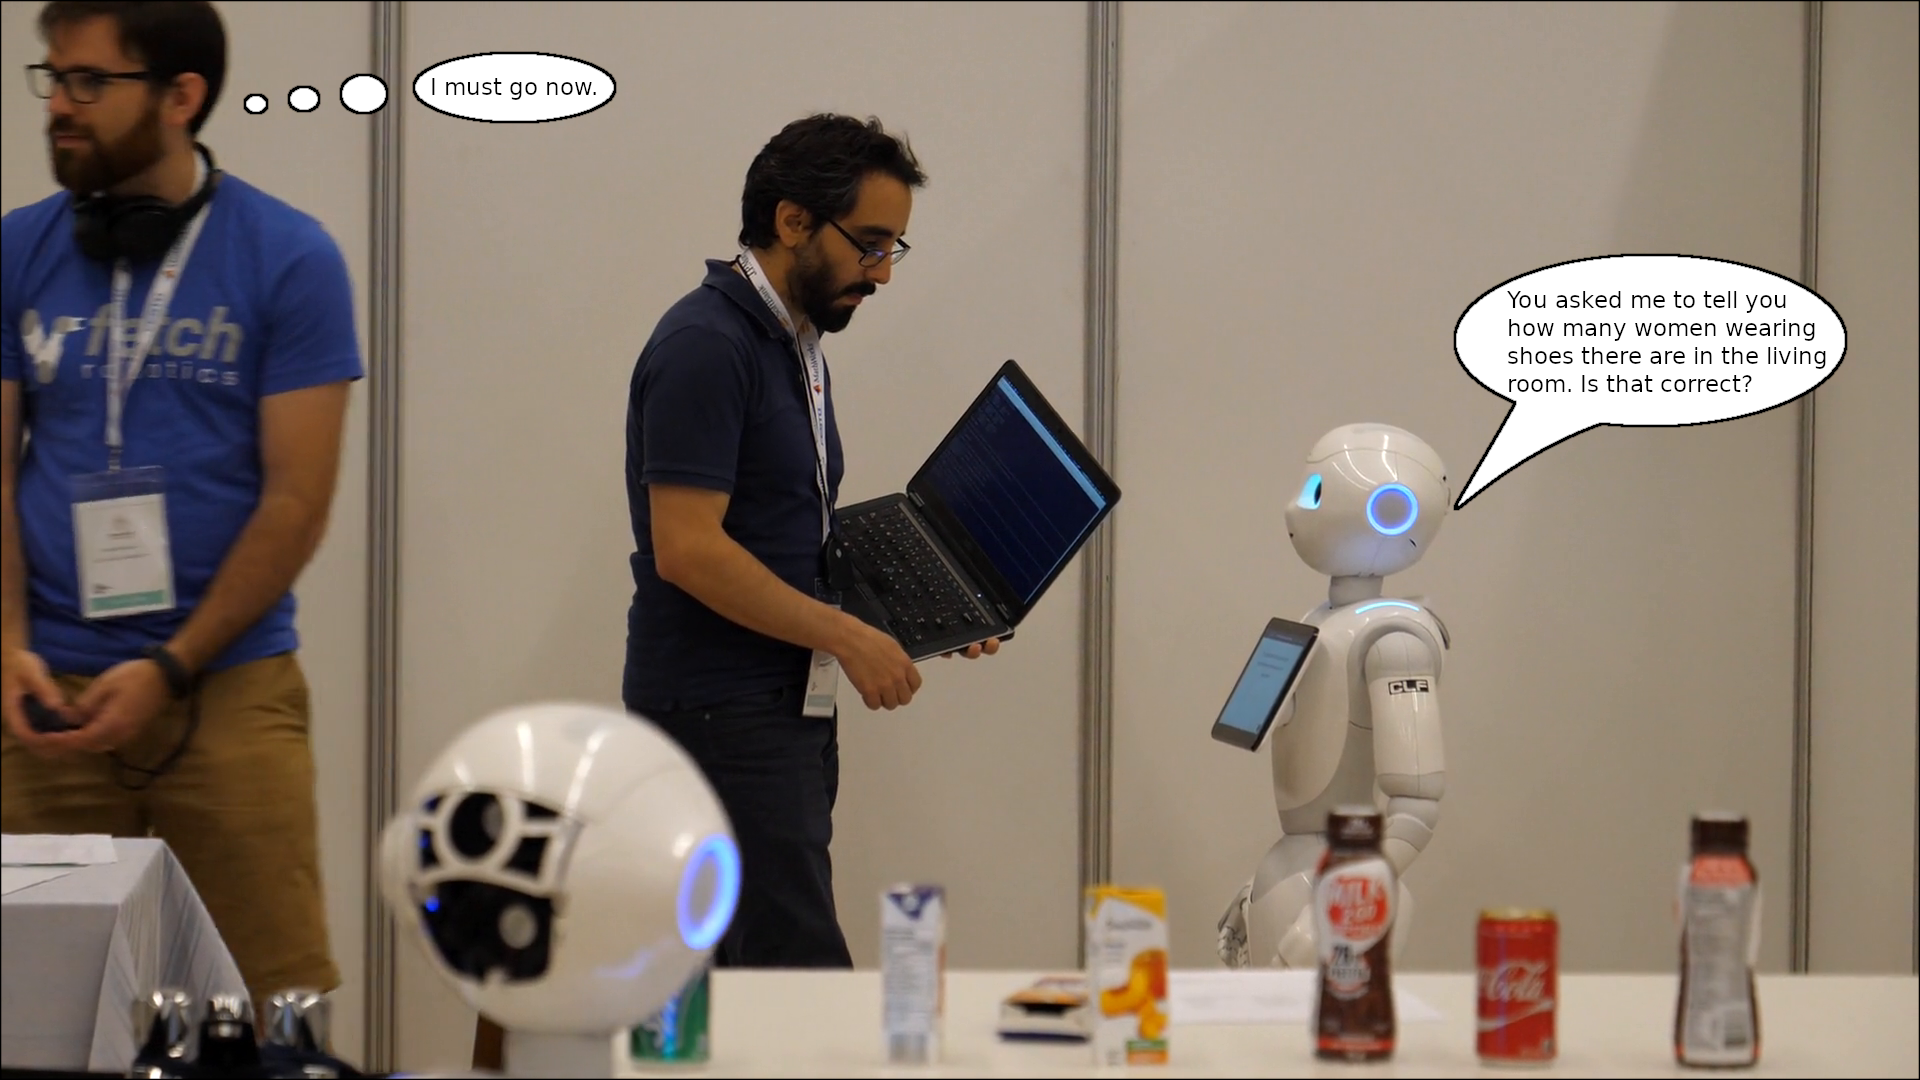
\includegraphics[width=.8\textwidth]{bilder/motivation/intro_2_edit.png}\\\vspace{3pt}
	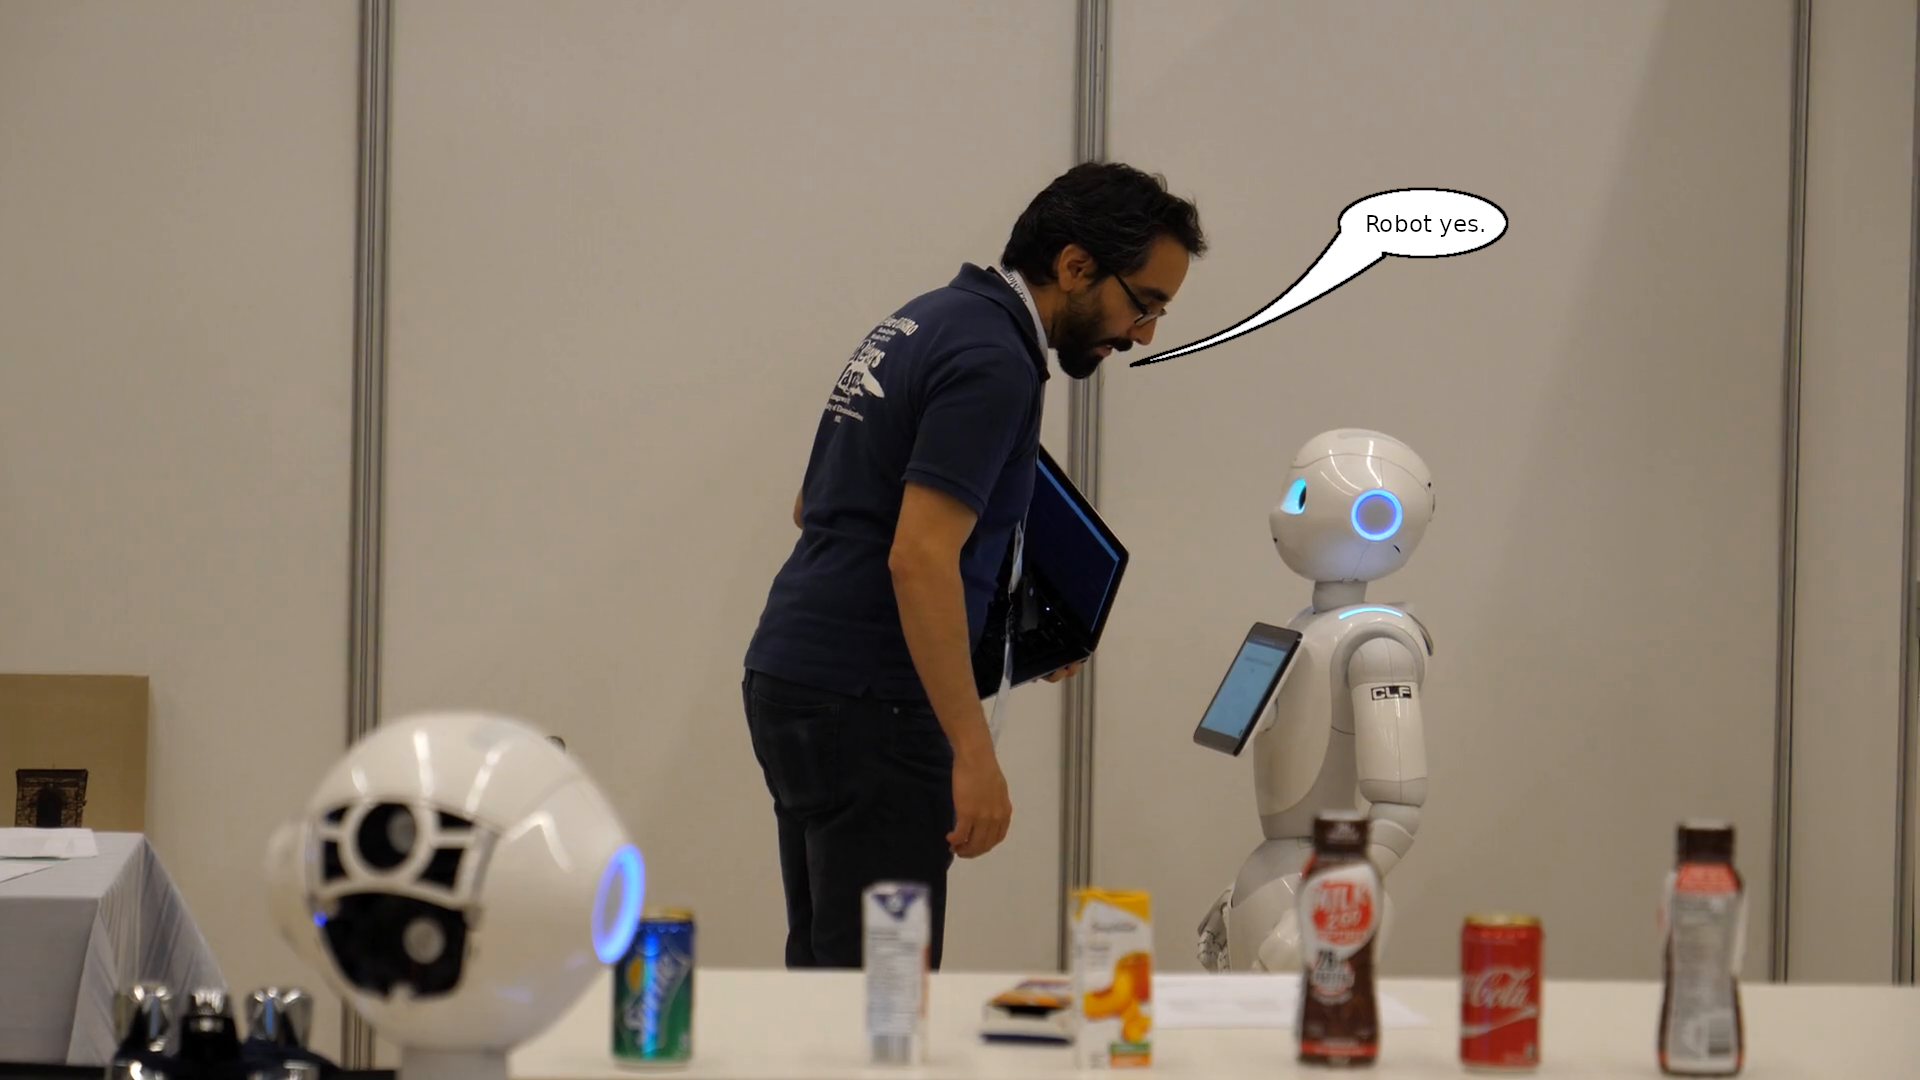
\includegraphics[width=.8\textwidth]{bilder/motivation/intro_3_edit.png}\\\vspace{3pt}
	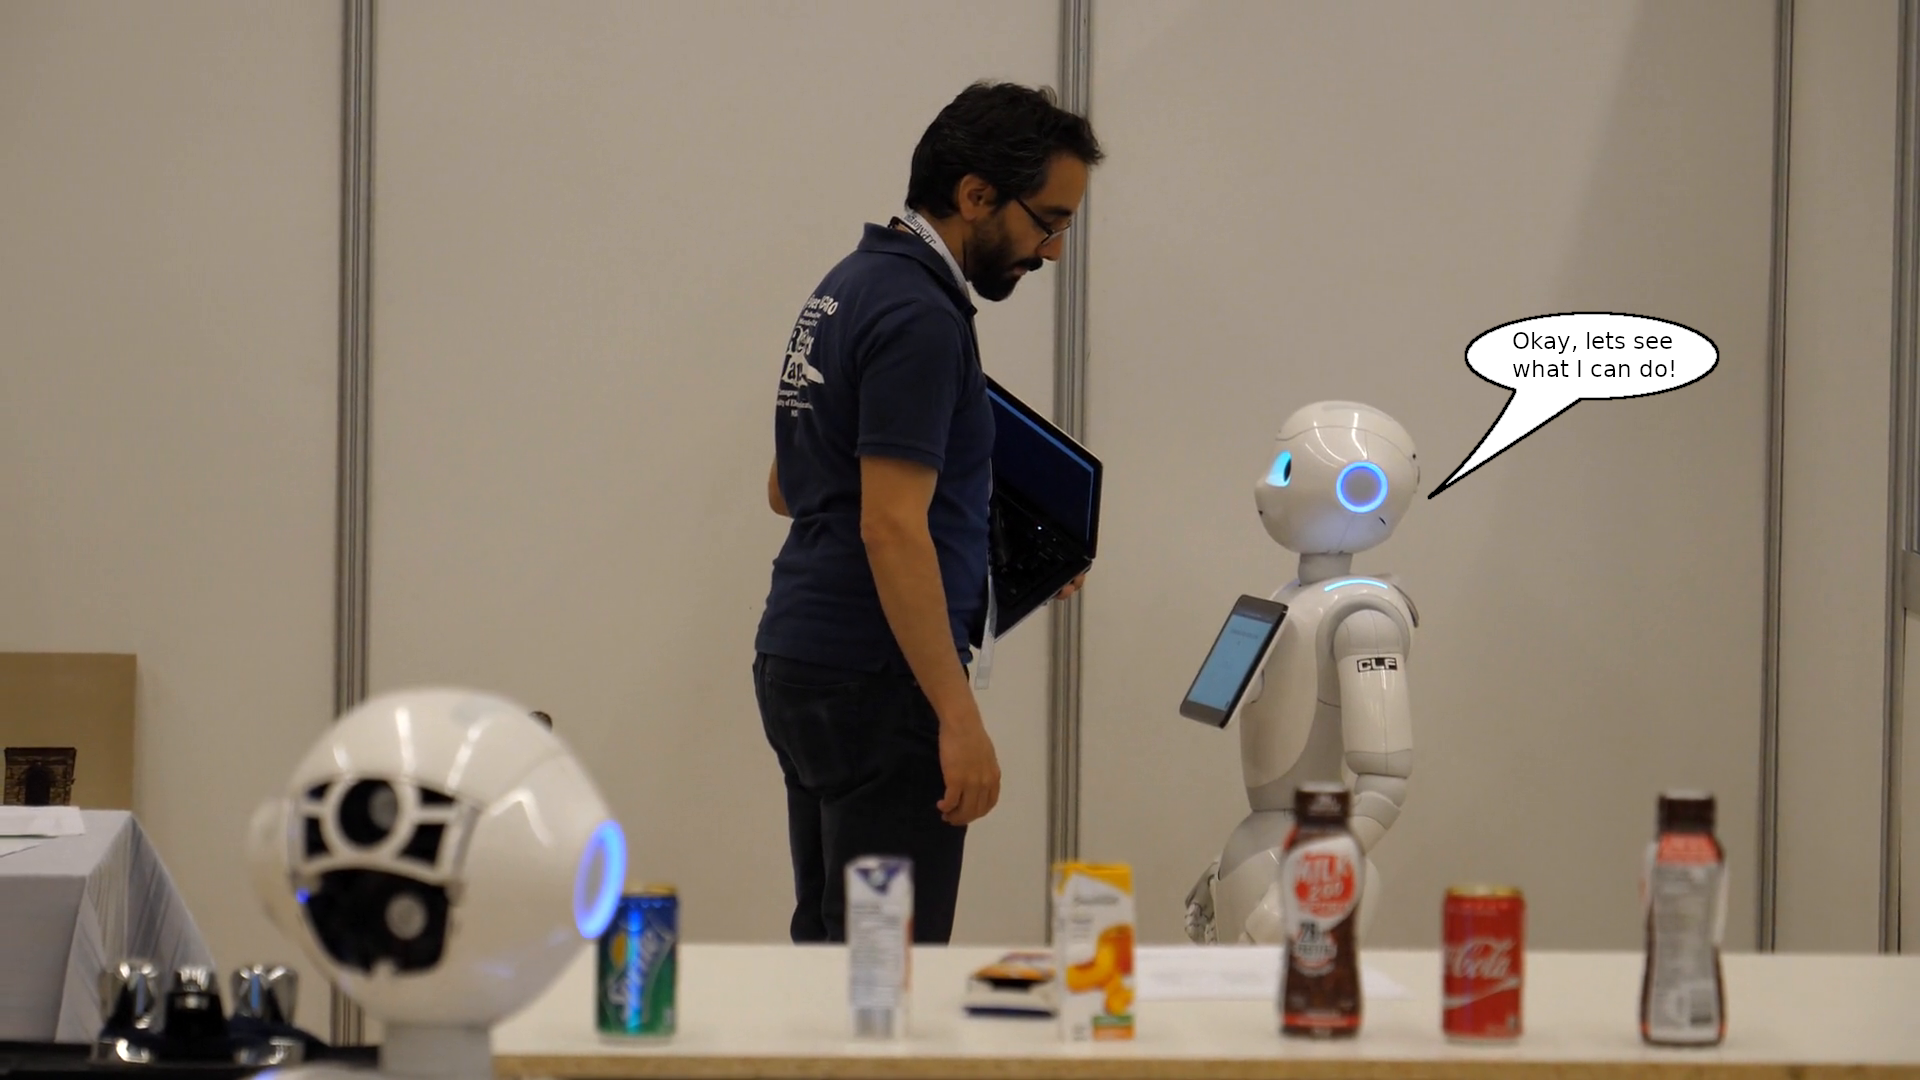
\includegraphics[width=.8\textwidth]{bilder/motivation/intro_4_edit.png}\\\vspace{3pt}
	
	\caption{Interaction between two referees and a robot in the RoboCup@home league.
		The referee in blue abandons the robot mid interaction, which does not acknowledge this at all.}
	\label{pic:moti:imustgonow}
\end{figure}

Therefore, the shown interactions appear unnatural:
the robot does not seem to perceive the human, instead it is quite clear that it just listens for a particular combination of words.
A similar phenomenon could very publicly be observed in the recent past, when Amazons Alexa ordered a variety of objects online, after hearing commands from a  TV commercial\footnote{\url{http://archive.is/zXuJu}}.
The solution employed by Amazon to stop this from happening with its own TV commercials seems to be a purposefully altered audio signal\footnote{\url{http://archive.is/d3uVu}} instead of a more general approach.

In the context of social robotics, these kinds of behavior are not desirable since approaches to partially solve these problems can be found in current literature \cite{opdenAkker:2009:YAR:1708376.1708379}.
Voice recognition technologies which can be used to differentiate speakers are available \cite{DBLP:journals/corr/abs-1003-4083}.
Additionally, computer vision is used to search for speakers, either standalone, looking for moving lips, or in combination with sound source localization (see \ref{basics:ssl}) \cite{1048137,lookwhostalking,840663,whosaidthat}.

Suitable robot behaviors need to be created, to take all this information into account.
When creating these behaviors, one must consider how the corresponding percepts are processed.
The behavior in question must either be able to combine the information, e.g. a spoken utterance and a distinct, detected voice or receive this information in a pre-combined manner.
If the behavior handles the combination, both may not be fed into the behavior at the same time, resulting in the problem to combine them.
A number of factors have to be considered when combining these information, e.g. Information may arrive asynchronous.
For example:
while just a single, long speech utterance may be received, a number of voices can be detected, or several results of the same voice.
Results in that sense are singular perceptions of a component, e.g. a voice recognizer or an \gls{ssl} detector.
Thus results have to be combined in a manner that takes this asynchrony into account.
Additionally, results will have different calculation times, based on what component created them and thus may be temporally unaligned.
This must be considered as well, creating the need to synchronize results based on their occurrence in time.

The problems just presented are clearly out of scope for robot behaviors an thus should be handled separately, due to their complexity.
I thus declare the \textbf{main goal of this thesis} to create a \textbf{framework for the automatic generation of these synchronized audio analysis results}.

Furthermore, a number of \textbf{secondary goals} can be declared.
Naturally any approach to synchronize audio results shall not have a negative impact on these results.
This can be specified in two more concrete terms.
First and foremost, the \textbf{accuracy of the results shall not decrease} by being incorporated in the proposed solution.
Second, synchronizing the \textbf{results shall not take considerably longer to compute} than not synchronizing them.
To put this into context: waiting for a result more than twice as long can not be deemed acceptable.

%---------------------------------- modularity secnd goal

Robotics is a field of intensive current research, and in the last years a number of leaps have been made.
These include, but are no limited to OpenPose \cite{cao2018openpose}, YOLO \cite{yolov3} and DeepSpeech \cite{deepspeech}.
Modularity and the ability to include such advances without the need to completely overhaul an existing system greatly decreases the time needed to incorporate such new technologies.
In turn, research speed can benefit.
I can thus declare an additional \textbf{secondary goal} in the form of \textbf{modularity}, to increase the usability of the proposed framework.

%-----------------------------------

The rest of this thesis is structured as follows:
I will first introduce concepts and frameworks in chapter \ref{basics:start}.
Here, first latency is introduced.
Latency is of special importance since it  plays a role in the computation times and is thus of particular interest with regards to the similar secondary goal.
After this I will discuss and briefly explain the concepts of \gls{asr}, \gls{ssl} and beamforming, as these can yield results of interest or be used to enhance audio signals, are partially incorporated in the later evaluation and will later present a number of challenges for the design of the proposed framework.
Finally I will explain \gls{ros}, a middleware used in the later proposed framework.

Thereafter I will present related work in chapter \ref{related:frameworks}, which will be divided in three parts.
First, a brief overview of a framework which focuses on \gls{ssl} and beamforming will be given.
Then I will discuss several fusion and synchronization approaches in preparation for my approach.
Lastly, an overview of current and former teams of the RoboCup@Home league, a prominent will be given, with special focus on their speech understanding and data fusion approaches.

After this I will present my solution in chapter \ref{main:main}.
Based on the goals formulated above and fusion approaches discussed in chapter \ref{related:fusion}, and in consideration of the concepts of latency and beamforming discussed in chapter \ref{basics:latency}, I will then present my approach for synchronization and fusion of speech analysis data.
This solution is a framework comprised of a library and a master component, the Orchestrator.
This chapter will close with an overview of the components developed over the course of this thesis.

I will then proceed to evaluate my proposed solution in chapter \ref{eval} based on two experiments.
The first experiment is conducted with the help of a data set, and is intended to evaluate the performance of the developed framework with regards to computation time.
The second experiment is heavily inspired by the ''Speech and Person Recognition'' Task of RoboCup@Home \cite{rulebook_2018}.
It is intended to evaluate the accuracy of the proposed framework in comparison to a pre-existing solution.
Both experiments will be able to show the main goal of this thesis to be achieved.
The data set experiment in particular will show the requested modularity.

Lastly I will summarize my findings and point out possible future work in chapter \ref{conclusion}.
The central point of this chapter is that due to the findings of chapter \ref{eval}, more and better components can be developed and the next step can be taken, i.e. behaviors equipped to handle situations such as those seen in figure \ref{pic:moti:imustgonow} by utilizing synchronized data can be created.

%In the appendix, I will detail the source code repositories as well as build and start instructions for the acrewed components.
%!TEX root = thesis.tex

\chapter{Related Work}

In this chapter a number of related projects and research findings will be presented and discussed. 
Several directions will be explored, i.e. an existing audio framework to transport audio \& create audio processing pipelines and different approaches to fusion of information.
Lastly RoboCup@Home, a competition between domestic robots with a strong research focus will be discussed, and several RoboCup@Home teams will be looked into with respect to their synchronization and fusion methods.

%!TEX root = ../../thesis.tex

\section{HARK}
\label{related:frameworks}
In this part \gls{hark} \cite{Nakadai_2017jrm} will be discussed, a modular framework with explicit focus on integrating beamforming and speech recognition solutions, developed by a team of researchers centered around Kyoto University.
Its goal is to provide an all in one solution for audition in robots specifically.
\gls{hark} is modular as it provides several algorithms (so called nodes) for each processing step.
These are centered around \gls{ssl}, beamforming, filtering, and feature extraction nodes.
\gls{hark} does not directly incorporate \gls{asr} solutions, but instead opts to extract audio features and send them via network to dedicated programs.
These are thusly not under its direct control.
It does not directly support other kinds of audio analysis, such as emotion-, voice-, or gender-recognition.
Nevertheless, one could develop these kinds of nodes to work with audio received via network and thus ''trick'' \gls{hark} to incorporate these nodes.
Naturally, it thus does not support the synchronization of results of any such components.
All the more, it does not support the synchronization of \gls{ssl} and \gls{asr} results, as results of \gls{asr} nodes lie outside its control.

\gls{hark} will take care of transporting audio data in between processing steps, but mostly transfers them in a frequency based representation, not as raw audio data.
This results in quite stripped down nodes, as it reduces the number of fast Fourier transforms needed to flat one instead of one per node relying on them.
Nodes which rely on raw audio however, must either manually restore the signal or use a specially developed node for this task.
Both variants results in a degrading signal however.

%-----------------------------------------------------------------------

%!TEX root = ../thesis.tex

\section{Fusion}
%!TEX root = ../../thesis.tex

\section{RoboCup@Home}
\label{related:robocup}
The RoboCup was founded in 1996 as an annual soccer competition for robots with the goal to beat the human world champions by 2050 (todo cite https://www.robocup.org/objective).
Over the years, RoboCup split into several leagues and expanded into other disciplines as well, such as the Rescue Robot league or the RoboCup@Work league.

RoboCup@Home (todo cite http://www.robocupathome.org/) is a league of the RoboCup dedicated to service robots in a domestic environment. % genauere beschreibung von @home, how is this relevant?
Therefore, human robot interaction is one of, if not the primary focus of this league.
Naturally, speech recognition systems are used as the default way to interact and communicate with the robots.
This results in the demand for robust speech recognition software.%, but also introduces problems rather unnoticed by theoretical research, such as...

One of the tasks tested in RoboCup@Home in 2017 and 2018, the ''Speech and Person Recognition'' task \cite{rulebook_2018}, is of particular interest for this work, as it mainly tests the basic speech recognition ability of the robots. 
As it was used in several RoboCup events over two years, and on dozens of robots, it is an convenient test to evaluate any speech recognition system on a robot.
Consequently, it will be used to evaluate the performance of the proposed pipeline later in chapter \ref{eval:task_start}, where the test will also be illustrated in greater detail. 

To gather information on the state of the art with regards to synchronization of sensor results and speech results in particular, I will provide an overview of established RoboCup@Home teams, which published information on that matter.
However, this information is relatively sparse in team description papers and on the teams websites, so some additional information was gathered by contacting the teams directly.

\subsection{SPQReL}
The SPQReL team from Sapienza University of Rome and the University of Lincoln use several fusion approaches. (todo cite)
Visual person perceptions were matched with \gls{ssl} results, based on their respective angular difference, and could thus be tagged as speaking.
Spoken sentences could then be mapped to speaking persons (according to email).
They employ several speech recognizers, i.e. Google Speech API and a Nuance speech recognizer, and fuse their results with a custom speech understanding system called \textit{LU4R} (todo cite), which is able to prioritize results based on expected domain specific terms. 
As such, this approach fits into the category of decision level techniques, as discussed in section \ref{related:fusion}.

\subsection{RoboFEI}
The RoboFEI team from Centro Universitário FEI in Sao Paolo (TODO cite) uses a specific microphone configuration to handle problems caused by moving sound source localization microphones.
Their robot's head is attached to a rotating pipe, which enables it to spin around its axis, while the robot's microphone array is attached to a static shaft running through that pipe which keeps it still.
As such, the position and movement of the robot's head are not relevant for sound source localization results and beamforming, and can as such be ignored.
Nevertheless, the robots own position and movement needs to be taken into account when performing \gls{ssl}, as is the case for all mobile robots.

\subsection{Tech United}
The Tech United team from the Eindhoven University of Technology provides some information about their speech recognition system.
In 2018, they generated \gls{ssl} information independently from their speech recognition.(TODO cite 2018 tdp)
They did not fuse these information however, instead opting to separately process them. %(mail)


\subsection{Walking Machine}
The Walking Machine team from École de Technologie Supérieure in Montreal (TODO cite) uses an solution, ODAS (TODO cite), which would enable them to perform \gls{ssl} and beamforming in one component, thus providing an enhanced audio signal.
However, they appear to only use its \gls{ssl} capabilities at this time.


\subsection{Kamerider}
The Kamerider team from Nankai University, China provides some information on the components they use for speech recognition and SSL (TODO cite).
They use Gstreamer to segment audio, which is then being processed by \gls{ps}.
Additionally, they use \gls{hark} for \gls{ssl}.
This way they appear to have modularized their components to a greater degree than other teams.
However, they gave no information about the interfacing of thusly acquired \gls{asr} and \gls{ssl} results.
%https://raw.githubusercontent.com/wiki/RoboCupAtHome/AtHomeCommunityWiki/files/tdp/2019-opl-kamerider_opl.pdf
 %(http://openbotics.org/kamerider/index.php?title=Main_Page)


\subsection{Hibikino Musashi}
%https://raw.githubusercontent.com/wiki/RoboCupAtHome/AtHomeCommunityWiki/files/tdp/2019-dspl-hibikino-musashiathome.pdf
The Hibikino-Musashi team of the Kyushu Institute of Technology also uses \gls{hark}, specifically its \textit{MUSIC} algorithm for \gls{ssl}.
Additionally, they employ an \gls{asr} solution in the form of \textit{Google SpeechRec} via its web API on the Chrome web browser.
We could however find no information about how the results of those components were interfaced.

\subsection{ToBi}
The team of Bielefeld (ToBi) of Bielefeld University can be discussed in greater detail, as I am a former member of this team.
For \gls{ssl} they used a proprietary solution which came with their Pepper robot %todo cite pepper and softbanks
while they used a \gls{ps} based component for \gls{asr}, the \gls{psa}. 

\gls{asr} and \gls{ssl} results are merged on the behavior layer, but only when \gls{ssl} information are explicitly needed.
The method with which they are merged is rather simplistic.
\gls{ssl} results are temporarily stored along a timestamp, which corresponds to the time these results were gathered.
Whenever an \gls{asr} result needs to be enhanced with \gls{ssl} results, an average is calculated over the \gls{ssl} results which were recorded between two and half a second before said \gls{asr} result.
This offset is employed to mitigate the time the \gls{psa} needs to recognize an utterance and the time needed by the behavior engine. 

The \gls{psa} is an \gls{asr} component which is based on \gls{ps}. \label{related_work:psa}
It captures sound directly from a microphone via \gls{alsa}, which is then segmented, to ensure only audio containing actual speech is evaluated.
It segments audio based on a loudness threshold, which, if crossed long enough, will start a segmentation.
This segmentation is ended either if a certain time limit is exceeded or if the loudness of received audio chunks drops under a second, typically slightly lower threshold.
Audio which is thus decided to contain speech will then be fed into \gls{ps}.
After a segmentation is ended, \gls{ps} will produce a result, which is then published via a \gls{ros} message.
We will use this component in later experiments (see chapters \ref{eval:dataset} and \ref{eval:task_start}).

One of these experiments will show the \gls{psa} to require considerably less time for recognitions than these 500ms.
However, a number of factors make this a good approximation still.
First, during the RoboCup@Home event, all computations are done on the robot itself, which sports considerably weaker hardware than the machine used for our experiments.
Additionally, the grammars typically used in RoboCup@Home Tasks are considerably bigger than the grammar used in our experiments, which makes matching a given utterance to a phrase in the grammar computationally more expensive.
%%!TEX root = thesis.tex

%=============================================================================


\chapter*{Statement of authorship}

I hereby certify that this thesis has been composed by me and is based on my own work unless stated otherwise. 
No other person’s work has been used without due acknowledgment in this thesis. 
All references and verbatim extracts have been quoted, and all sources of information, including graphs and data sets, have been specifically acknowledged. 
This thesis has not been presented to an examination office in the same or a similar form yet.
\\\\\\\\
Bielefeld, \today
\\\\\\\\
Robert Feldhans

%=============================================================================

\backmatter
%\printglossaries
\printbibliography[heading=bibintoc]

%\appendix
%\input{app_a}

\end{document}